\xiti
\begin{xiaotis}

\xiaoti{已知: 矩形 $ABCD$, $M$ 是 $BC$ 的中点, $BC = 2 AB$。
    求证: $MA \perp MD$。
}

\xiaoti{矩形对角线组成的对顶角中, 有一组是 $60^\circ$, 对角线与各边组成的角是多少度?}

\xiaoti{已知: $O$ 是矩形 $ABCD$ 对角线的交点,$E$、$F$、$G$、$H$ 分别是 $AO$、$BO$、$CO$、$DO$
    上的一点, 并且 $AE = BF = CG = DH$。
    求证: 四边形 $EFGH$ 是矩形。
}

\xiaoti{求证:两条平行线与第三条直线相交, 两组内错角的平分线相交所成的四边形是矩形。}

\xiaoti{求作矩形 $ABCD$,使 $AB = a$, $AC = b$。}

\begin{figure}[htbp]
    \centering
    \begin{minipage}[b]{4cm}
        \centering
        \begin{tikzpicture}
	\tkzDefPoints{0/0/b1, 3/0/b2, 0/1/a1, 2/1/a2}
	\tkzDrawSegments[xianduan={below=0pt}](b1,b2  a1,a2)
	\tkzLabelSegment[above](a1,a2){$a$}
	\tkzLabelSegment[above](b1,b2){$b$}
\end{tikzpicture}


        \caption*{(第 5 题)}
    \end{minipage}
    \qquad
    \begin{minipage}[b]{4.5cm}
        \centering
        \begin{tikzpicture}
    \tkzDefPoints{0/0/B, 3/0/C, 1.5/2.7/A}
    \tkzDefMidPoint(B,C)  \tkzGetPoint{M}
    \tkzDefLine[altitude](A,M,B)  \tkzGetPoint{G}
    \tkzDefLine[altitude](A,M,C)  \tkzGetPoint{D}
    \tkzDefLine[altitude](A,G,C)  \tkzGetPoint{F}
    \tkzDefLine[altitude](A,D,B)  \tkzGetPoint{E}
    \tkzInterLL(G,F)(D,E)  \tkzGetPoint{H}
    \tkzDrawPolygon(A,B,C)
    \tkzDrawSegments(M,G  G,F  M,D  D,E)
    \tkzMarkRightAngle(B,G,M)
    \tkzMarkRightAngle(B,E,D)
    \tkzMarkRightAngle(C,D,M)
    \tkzMarkRightAngle(C,F,G)
    \tkzLabelPoints[above](A,H)
    \tkzLabelPoints[left](B,G,E)
    \tkzLabelPoints[right](C,D,F)
    \tkzLabelPoints[below](M)
\end{tikzpicture}


        \caption*{(第 7 题)}
    \end{minipage}
    \qquad
    \begin{minipage}[b]{5.2cm}
        \centering
        \begin{tikzpicture}
    \tkzDefPoints{0/0/B, 4/0/C, 0/4/A, 4/4/D}

    \tkzDefMidPoint(A,B)  \tkzGetPoint{L1}
    \tkzDefMidPoint(B,C)  \tkzGetPoint{B1}
    \tkzDefMidPoint(C,D)  \tkzGetPoint{R1}
    \tkzDefMidPoint(D,A)  \tkzGetPoint{A1}
    \tkzInterLL(A1,B1)(L1,R1)  \tkzGetPoint{O1}

    \tkzDefMidPoint(A1,O1)  \tkzGetPoint{L2}
    \tkzDefMidPoint(O1,R1)  \tkzGetPoint{B2}
    \tkzDefMidPoint(R1,D)   \tkzGetPoint{R2}
    \tkzDefMidPoint(D,A1)   \tkzGetPoint{A2}
    \tkzInterLL(A2,B2)(L2,R2)  \tkzGetPoint{O2}

    \tkzDefMidPoint(A2,O2)  \tkzGetPoint{L3}
    \tkzDefMidPoint(O2,R2)  \tkzGetPoint{B3}
    \tkzDefMidPoint(R2,D)   \tkzGetPoint{R3}
    \tkzDefMidPoint(D,A2)   \tkzGetPoint{A3}
    \tkzInterLL(A3,B3)(L3,R3)  \tkzGetPoint{O3}

    \tkzDrawPolygon(A,B,C,D)
    \tkzDrawSegments(A1,B1  L1,R1)
    \tkzDrawSegments(A2,B2  L2,R2)
    \tkzDrawSegments(A3,B3  L3,R3)
    \tkzFillPolygon[pattern={mylines[angle=45, distance={2pt}]}](A3,O3,R3,D)

    \tkzLabelPoints[left](A,B)
    \tkzLabelPoints[right](C,D)
\end{tikzpicture}


        \caption*{(第 11 题)}
    \end{minipage}
\end{figure}


\xiaoti{求证: 如果菱形的一个角是 $120^\circ$, 那么从这个角的顶点向对的两边所引两条垂线分别平分这两边。}

\xiaoti{已知: $\triangle ABC$ 中,$AB = AC$, $M$ 为 $BC$ 的中点, $MG \perp AB$,
    $MD \perp AC$, $GF \perp AC$, $DE \perp AB$, 垂足分别为 $G$、$D$、$F$、$E$,
    $GF$、$DE$ 相交于 $H$。求证: 四边形 $HGMD$ 是菱形。
}

\xiaoti{$O$ 是矩形 $ABCD$ 的对角线的交点, 作 $DE \pingxing AC$, $CE \pingxing BD$,
    $DE$、$CE$ 交于 $E$。 求证: 四边形 $OCED$ 是菱形。
}

\xiaoti{画菱形 $ABCD$, 使 $AC = 50\;\haomi$, $\angle BAD = 60^\circ$。}

\xiaoti{已知: 在 $\triangle ABC$ 中, $\angle C = 90^\circ$, $CD$ 是角平分线,$DE \perp BC$,
    $DF \perp AC$, 垂足分别是 $E$、$F$。 求证:四边形 $ABCD$ 是正方形。
}

\xiaoti{已知正方形 $ABCD$, $AB = 24\;\limi$,对边中点的连线将正方形分成四个小正方形,
    再同样分下去,分三次所得的正方形的周长是多少?
}

\xiaoti{求证: 正方形的两条对角线把正方形分成四个全等的等腰直角三角形。}

\xiaoti{求证: 矩形的各内角平分线组成的四边形是正方形。}

\xiaoti{求证: 依次连结正方形各边的中点所成四边形为正方形。}

\xiaoti{以一条已知线段为对角线,求作正方形。}

\xiaoti{填充下列定理中所缺的词:}
\begin{xiaoxiaotis}

    \xxt{两条对角线 \xhx[5cm] 的平行四边形是矩形;}

    \xxt{两条对角线 \xhx[5cm] 的四边形是矩形;}

    \xxt{两条对角线 \xhx[5cm] 的平行四边形是菱形;}

    \xxt{两条对角线 \xhx[5cm] 的四边形是菱形;}

    \xxt{两条对角线 \xhx[5cm] 的矩形是正方形;}

    \xxt{两条对角线 \xhx[5cm] 的菱形是正方形;}

    \xxt{两条对角线 \xhx[5cm] 的平行四边形是正方形;}

    \xxt{两条对角线 \xhx[5cm] 的四边形是正方形。}
\end{xiaoxiaotis}


\xiaoti{求作:}
\begin{xiaoxiaotis}

    \xxt{已知点 $A$ 关于点 $O$ 的对称点;}

    \xxt{已知线段 $AB$ 关于点 $O$ 的对称线段;}

    \xxt{已知 $\triangle ABC$ 关于点 $O$ 的对称三角形。}

\end{xiaoxiaotis}


\xiaoti{作一个与已知四边形 $ABCD$ 中心对称的四边形。}
\begin{xiaoxiaotis}

    \xxt{以顶点 $A$ 为对称中心;}

    \xxt{以 $BC$ 边的中点 $O$ 为对称中心。}

\end{xiaoxiaotis}


\xiaoti{作已知线段 $AB$ 关于点 $O$ (不在 $AB$上)的对称线段 $A'B'$。
    再作 $A'B'$ 关于点 $O'$(不在 $A'B'$ 上) 的对称线段 $A''B''$。
    并证明:$A''B'' \pingxing AB$。
}

\xiaoti{求证: 任何一个具有对称中心的四边形是平行四边形。(用中心对称证明。)}

\xiaoti{已知: 直线 $x$、$y$ 互相垂直,垂足为 $O$。
    作线段 $AB$ 关于轴 $x$ 的对称线段 $A'B'$,
    再作 $A'B'$ 关于轴 $y$ 的对称线段 $A''B''$。
    线段 $AB$ 和 $A''B''$ 是否关于点 $O$ 对称?
}

\end{xiaotis}

